\documentclass{math}

\usepackage{graphicx}
\usepackage{pgfplots}
\pgfplotsset{compat=1.13}

\geometry{letterpaper, margin=0.5in}

\title{Differential Equations: Homework 2}
\author{Alvin Lin}
\date{January 2018 - May 2018}

\begin{document}

\maketitle
\clearpage

\section*{Section 1.3}

\subsubsection*{Exercise 1}
The direction field for \( \ddiff{y}{x} = \frac{4x}{y} \) is shown.
Verify that the straight lines \( y = \pm2x \) are solution curves, provided
\( x \ne 0 \).
\begin{align*}
  y &= 2x \\
  \ddiff{y}{x} &= 2 = \frac{4x}{y} = \frac{4x}{2x} = 2 \\
  y &= -2x \\
  \ddiff{y}{x} &= -2 = \frac{4x}{y} = \frac{4x}{-2x} = -2
\end{align*}
Sketch the solution curve with initial condition \( y(0) = 2 \). \\[1cm]
\begin{minipage}[class]{7cm}
  \begin{align*}
    \ddiff{y}{x} &= \frac{4x}{y} \\
    y\diff{y} &= 4x\diff{x} \\
    \int y\diff{y} &= \int 4x\diff{x} \\
    y^2 &= 2x^2+c \\
    y(0) &= 2 \quad c = 4 \\
    y^2 &= 2x^2+4
  \end{align*}
\end{minipage}
\begin{minipage}[c]{8cm}
  \begin{tikzpicture}[scale=0.8]
    \begin{axis}[axis lines=middle]
      \addplot[blue] {(2*x^2+4)^0.5};
      \addplot[blue] {-(2*x^2+4)^0.5};
    \end{axis}
  \end{tikzpicture}
\end{minipage}
\clearpage

Sketch the solution curve with initial condition \( y(2) = 1 \). \\[1cm]
\begin{minipage}[c]{8cm}
  \begin{align*}
    \ddiff{y}{x} &= \frac{4x}{y} \\
    y\diff{y} &= 4x\diff{x} \\
    \int y\diff{y} &= \int 4x\diff{x} \\
    y^2 &= 2x^2+c \\
    y(2) &= 1 \quad c = -7 \\
    y^2 &= 2x^2-7
  \end{align*}
\end{minipage}
\begin{minipage}[c]{8cm}
  \begin{tikzpicture}[scale=0.8]
    \begin{axis}[axis lines=middle, samples=200]
      \addplot[blue,domain={-4:-2}] {(2*x^2-7)^0.5};
      \addplot[blue,domain={2:4}] {(2*x^2-7)^0.5};
      \addplot[blue,domain={-4:-2}] {-(2*x^2-7)^0.5};
      \addplot[blue,domain={2:4}] {-(2*x^2-7)^0.5};
    \end{axis}
  \end{tikzpicture}
\end{minipage} \\[0.5cm]
What can you say about the behavior of the above solutions as \( x\to+\infty \)?
How about \( x\to-\infty \)? \\
As \( x \) approaches positive/negative infinity, the solutions become more and
more vertical. This makes sense since the slope approaches positive and
negative infinity.

\subsubsection*{Exercise 3}
A model for the velocity \( v \) at time \( t \) of a certain object falling
under the influence of gravity in a viscous medium is given by the equation
\[ \ddiff{v}{t} = 1-\frac{v}{8} \]
From the direction field, sketch the solutions with the initial conditions
\( v(0) = 5, 8, 15 \). Why is the value \( v = 8 \) called the ``terminal
velocity''?
\begin{center}
  \begin{tikzpicture}[scale=1.5]
    \begin{axis}[axis lines=middle,ymin=-2,ymax=18,ytick={5,8,15}]
      \addplot[->,red] {8};
      \addplot[->,red] {-(e^((-x/8)+1.09))+8};
      \addplot[->,red] {7*e^(-x/8)+8};
    \end{axis}
  \end{tikzpicture}
\end{center}
\( v = 8 \) is called the terminal velocity because no object can cross that
line from either side. All objects will eventually accelerate or decelerate
to \( v = 8 \) from any initial velocity. It represents the maximum velocity
that an object can freefall at in the viscous medium.

\subsubsection*{Exercise 5}
The logistic equation for the population (in thousands) of a certain species is
given by:
\[ \ddiff{p}{t} = 3p-2p^2 \]
\begin{center}
  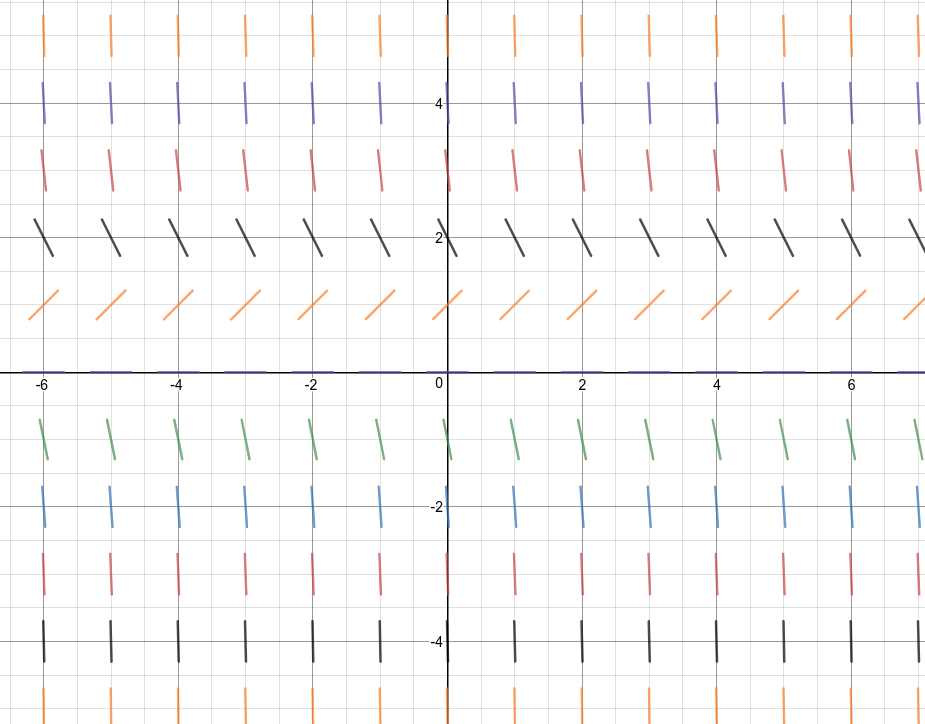
\includegraphics[width=16cm]{assets/hw_02_01.png}
\end{center}
If the initial population is 3000, what can you say about the limiting
population \( \lim_{t\to+\infty}p(t) \)?
\[ \lim_{t\to+\infty}p(t) = 1500 \]
If \( p(0) = 0.8 \), what is \( \lim_{t\to+\infty}p(t) \)?
\[ \lim_{t\to+\infty}p(t) = 1500 \]
Can a population of 2000 ever decline to 800? \\
No, the population will stop decreasing at 1500.


\section*{Section 1.4}

\subsubsection*{Exercise 5}
Use Euler's method with step size \( h = 0.1 \) to approximate the solution to
the initial value problem
\[ y' = x-y^2 \quad y(1) = 0 \]
at the points \( x = 1.1, 1.2, 1.3, 1.4, 1.5 \).
\begin{center}
  \begin{tabular}{|c|c|}
    \hline
    \( x_0 = 1 \) & \( y_0 = 1 \) \\
    \hline
    \( x_1 = 1.1 \) & \( y_1 = 1+0.1(1-1^2) = 1 \) \\
    \hline
    \( x_2 = 1.2 \) & \( y_2 = 1+0.1(1.1-1^2) = 1.01 \) \\
    \hline
    \( x_3 = 1.3 \) & \( y_3 = 1.01+0.1(1.2-1.01^2) = 1.028 \) \\
    \hline
    \( x_4 = 1.4 \) & \( y_4 = 1.028+0.1(1.3-1.028^2) = 1.052 \) \\
    \hline
    \( x_5 = 1.5 \) & \( y_5 = 1.052+0.1(1.4-1.052^2) = 1.081 \) \\
    \hline
  \end{tabular}
\end{center}

\section*{Section 2.2}

\subsubsection*{Exercise 3}
Determine whether the given differential equation is separable.
\begin{align*}
  \ddiff{s}{t} &= t\ln(s^{2t})+8t^2 \\
  &= 2t^2\ln(s)+8t^2 \\
  &= 2t^2(\ln(s)+4) \\
  \frac{1}{\ln(s)+4}\diff{s} &= 2t^2\diff{t}
\end{align*}

\subsubsection*{Exercise 7}
Solve the equation:
\begin{align*}
  x\diff{y}{x} &= \frac{1}{y^3} \\
  y^3\diff{y} &= \frac{1}{x}\diff{x} \\
  \int y^3\diff{y} &= \int\frac{1}{x}\diff{x} \\
  \frac{y^4}{4} &= \ln|x|+c
\end{align*}

\subsubsection*{Exercise 9}
Solve the equation:
\begin{align*}
  \ddiff{x}{t} &= \frac{t}{x\e^{t+2x}} \\
  x\e^{t+2x}\diff{x} &= t\diff{t} \\
  x\e^t\e^{2x}\diff{x} &= t\diff{t} \\
  x\e^{2x}\diff{x} &= \frac{t}{\e^t}\diff{t} \\
  \int x\e^{2x}\diff{x} &= \int\frac{t}{\e^t}\diff{t} \\
  x\e^x-\e^x &= -t\e^{-t}-\e^{-t}+c
\end{align*}

\subsubsection*{Exercise 12}
Solve the equation:
\begin{align*}
  \ddiff{y}{x} &= \frac{\sec^2(y)}{1+x^2} \\
  \frac{1}{\sec^2(y)}\diff{y} &= \frac{1}{1+x^2}\diff{x} \\
  \int\cos^2(y)\diff{y} &= \int\frac{1}{1+x^2}\diff{x} \\
  \frac{x}{2}+\frac{\sin(y)\cos(y)}{2} &= \arctan(x)+c
\end{align*}

\subsubsection*{Exercise 15}
Solve the equation:
\begin{align*}
  (x+xy^2)\diff{x}+\e^{x^2}y\diff{y} &= 0 \\
  x(1+y^2)\diff{x} &= -\e^{x^2}y\diff{y} \\
  -\frac{x}{\e^{x^2}}\diff{x} &= \frac{y}{1+y^2}\diff{y} \\
  -\int\frac{x}{\e^{x^2}}\diff{x} &= \int\frac{y}{1+y^2}\diff{y} \\
  \frac{-1}{2\e^{x^2}}+c &= \frac{\ln|y^2+1|}{2}
\end{align*}

\subsubsection*{Exercise 17}
Solve the initial value problem \( \ddiff{y}{x} = (1+y^2)\tan(x) \) with
\( y(0) = \sqrt{3} \):
\begin{align*}
  \ddiff{y}{x} &= (1+y^2)\tan(x) \\
  \frac{1}{1+y^2}\diff{y} &= \tan(x)\diff{x} \\
  \int\frac{1}{1+y^2}\diff{y} &= \int\tan(x)\diff{x} \\
  \arctan(y) &= -\ln|\cos(x)|+c \\
  \arctan(\sqrt{3}) &= -\ln|\cos(0)|+c \\
  \frac{\pi}{3} &= c \\
  \arctan(y) &= -\ln|\cos(x)|+\frac{\pi}{3}
\end{align*}
\clearpage

\subsubsection*{Exercise 19}
Solve the initial value problem \( \frac{1}{2}\ddiff{y}{x} =
\sqrt{y+1}\cos(x) \) with \( y(\pi) = 0 \):
\begin{align*}
  \frac{1}{2}\ddiff{y}{x} &= \sqrt{y+1}\cos(x) \\
  \frac{1}{2\sqrt{y+1}}\diff{y} &= \cos(x)\diff{x} \\
  \int\frac{1}{2\sqrt{y+1}}\diff{y} &= \int\cos(x)\diff{x} \\
  \sqrt{y+1} &= \sin(x)+c \\
  \sqrt{1} &= \sin(\pi)+c \\
  c &= 1 \\
  y &= (\sin(x)+1)^2-1
\end{align*}

\subsubsection*{Exercise 21}
Solve the initial value problem \( \frac{1}{\theta}\ddiff{y}{\theta} =
\frac{y\sin\theta}{y^2+1} \) with \( y(\pi) = 1 \):
\begin{align*}
  \frac{1}{\theta}\ddiff{y}{\theta} &= \frac{y\sin\theta}{y^2+1} \\
  \frac{y^2+1}{y}\diff{y} &= \theta\sin\theta\diff{\theta} \\
  \int\frac{y^2+1}{y}\diff{y} &= \int\theta\sin\theta\diff{\theta} \\
  \frac{y^2}{2}+\ln|y| &= \sin\theta-\theta\cos\theta+c \\
  \frac{1^2}{2}+\ln|1| &= \sin\pi-\pi\cos\pi+c \\
  \frac{1}{2}+0 &= 0+\pi+c \\
  c &= \frac{1}{2}-\pi \\
  \frac{y^2}{2}+\ln|y| &= \sin\theta+\theta\cos\theta+\frac{1}{2}-\pi
\end{align*}

\subsubsection*{Exercise 23}
Solve the initial value problem \( \ddiff{y}{t} = 2t\cos^2(y) \) with \( y(0) =
\frac{\pi}{4} \).
\begin{align*}
  \ddiff{y}{t} &= 2t\cos^2(y) \\
  \sec^2(y)\diff{y} &= 2t\diff{t} \\
  \int\sec^2(y)\diff{y} &= \int 2t\diff{t} \\
  \tan(y) &= t^2+c \\
  \tan(\frac{\pi}{4}) &= 0+c \\
  c &= 1 \\
  \tan(y) &= t^2+1 \\
  y &= \arctan(t^2+1)
\end{align*}

\subsubsection*{Exercise 24}
Solve the initial value problem \( \ddiff{y}{x} = 8x^3\e^{-2y} \) with \( y(1) =
0 \).
\begin{align*}
  \ddiff{y}{x} &= 8x^3\e^{-2y} \\
  \e^{2y}\diff{y} &= 8x^3\diff{x} \\
  \int\e^{2y}\diff{y} &= \int 8x^3\diff{x} \\
  \frac{\e^{2y}}{2} &= 2x^4+c \\
  \frac{\e^0}{2} &= 2(1^4)+c \\
  c &= -\frac{3}{2} \\
  \e^{2y} &= 4x^4-3 \\
  y &= \frac{\ln(4x^4-3)}{2}
\end{align*}

\subsubsection*{Exercise 26}
Solve the initial value problem \( \sqrt{y}\diff{x}+(1+x)\diff{y} = 0 \) with
\( y(0) = 1 \).
\begin{align*}
  \sqrt{y}\diff{x}+(1+x)\diff{y} &= 0 \\
  (1+x)\diff{y} &= -\sqrt{y}\diff{x} \\
  -y^{-\frac{1}{2}}\diff{y} &= \frac{1}{1+x}\diff{x} \\
  -\int y^{-\frac{1}{2}}\diff{y} &= \int\frac{1}{1+x}\diff{x} \\
  -2\sqrt{y} &= \ln|1+x|+c \\
  -2\sqrt{1} &= \ln|1|+c \\
  -2 &= c \\
  -2\sqrt{y} &= \ln|1+x|-2 \\
  y &= \bigg(\frac{\ln|1+x|-2}{-2}\bigg)^2
\end{align*}

\begin{center}
  If you have any questions, comments, or concerns, please contact me at
  alvin@omgimanerd.tech
\end{center}

\end{document}
